\chapter{GIRG generation}
\section{GIRGs definition}
We outline the key elements of GIRGs and the main variations and how they fit into a wider context of random graph models.

The GIRG definition according to \cite{bringmann2019geometric} is a random graph model defined by the edge connection probabilities

TODO below (div by n, infty norm) is what I had before, but in fact bringmann2019geometric uses below with div by W and ambiguous norm.
\begin{equation}
    p_{uv} = \Theta \left ( \min \left \{ 
        1,
        c \left (
            \frac{w_u w_v}{ n \norm{x_u - x_v}_\infty^d}
        \right )^\alpha    
    \right \}
    \right )
\end{equation}

\begin{equation}
    p_{uv} = \Theta \left ( \min \left \{ 
        1,
        c \left (
            \frac{w_u w_v / W}{\norm{x_u - x_v}^d}
        \right )^\alpha    
    \right \}
    \right )
\end{equation}

where $(w_u)_{u \in V}$ are node specific weights and $(x_u \in \chi)_{u \in V}$ are positions in some geometric space $\chi$, generally taken to be the d-dimensional torus or cube of side length 1.

This edge probability has a geometric factor from the distance $r_{uv} = \norm{x_u - x_v}_\infty$, and is proportional to $r_{uv}^{-d \alpha}$, where $\alpha > 0$, meaning that close by nodes are more likely to be connected. The $n^{-1}$ normalising factor ensures that as $n \to \infty$, expected node degrees are unchanged.

We often write $\rho_{uv} = \left ( \frac{w_u w_v / W}{\norm{x_u - x_v}^d} \right )$ to save on writing.

\paragraph{power law degree sequence} Like Chung-Lu, the weight sequences are usually assumed to follow a powerlaw distribution with an exponent $\tau \in (2, 3)$ (at least within some tolerance and in the large weight tail).
\begin{align*}
\eqname{exact power law distribution}
& W \sim \powerlaw(\tau)
\\
\eqname{pdf (default $x_{\min } = 1$)}
& p(w) = w^{-\tau} \text{ for } w \in [x_{\min }, \infty]
\\
& p(W \geq w) \propto w^{1 - \tau}
\end{align*}
% A general In practice a power law degree sequence is required to have a looser version of $\# \{w_u | w_u \geq w\} = \Theta(w^{1 - \tau})$.
This is a heavy tailed distribution (heavier than exponentially decaying tails). $\tau > 2$ is important to ensure that $E[W] = \Theta(1)$. This means that although we may in a sequence of $w_1, ..., w_n$ have some very large $w_i$, still the majority of the total weight is in the small valued $w_i$'s. 


\paragraph{Similarity to Chung-Lu} A key property of the GIRG model is that marginalising over possible node locations gives that $E_{x_v}[p_{uv} | x_u, w_u, w_v] = \Theta(\min\{1, \frac{w_u w_v}{n} \})$, which matches the Chung-Lu GGM. This means that many results for Chung-Lu carry through automatically into GIRGs, like simple facts that $E[d_u] = \Theta(w_u)$ (the expected degree of a node of a fixed weight is proportional to that weight). For this to hold we actually need to have $\alpha > 1$ - otherwise there are too many long distance edges. Essentially $\alpha > 1$ depresses the number of long distance edges to be $\Theta(\min\{1, \frac{w_u w_v}{W} \})$. No matter how large $\alpha$ is, there will always be $\Theta(\min\{1, \frac{w_u w_v}{W} \})$ short distance edges: $u \sim v$ where $p_{uv} = 1$.

\paragraph{Geometry} The exact geometry $\chi$, and the distance function $\norm{\cdot}$ can vary a great deal without affecting the key properties of GIRGs. $\chi = \T_d$ the d-dimensional torus is very handy for proofs, as the viewpoint of any node $x_u$ is equivalently at the "centre" of the space. For real applications the d-dimensional cube $\chi = [0, 1]^d$ can be more realistic, but then if $x_u$ is at the edge of the cube it has a different viewpoint to a node more at the centre of the cube.

Taking $\norm{\cdot} = \norm{\cdot}_\infty$ is also useful, but can be replaced equivalently by euclidean or other norms. The minimum component distance $\norm{x} = \min_i |x_i|$ is not a norm, but still holds retains most of the GIRG properties. This can make sense in that two nodes might have a higher edge probability by being close in one dimension, rather than every dimension.

The reason for the power of $d$ in $r_{uv}^d$ is to keep the edge probabilties equivalent with respect to the volume of space in different dimensions. The more general formula replaces replaces $||x_u - x_v||^d = r_{uv}^d$ with $Vol(B_r)$ the volume of the ball of radius $r=r_{uv}$.
For norms, $Vol(B_r) = \Theta(r^d)$, e.g. in the $\infty$-norm, $Vol(B_r) = (2r)^d$ as a cube with side-length $2r$. The euclidean ball has some $\pi$'s in the formula. For the minimum component distance, $Vol(B_r) = \Theta(r)$. Volumetric equivalence makes sense in that the edge probability $p_{uv} | x_u, w_u, w_v$ in the Torus is determined by integrating $\int_{r=0}^{r=1} p_{uv}(r) p(r) dr = \int_{Vol=0}^{Vol=1} p_{uv}(Vol) dVol$, where $Vol(r) = Vol(B_r)$ is the volume of the ball of radius $r$. Hence across different GIRGs of different dimensions $d$, keeping $p_{uv}(Vol)$ the same function therefore keeps the pairwise edge probabilities $p_{uv}$ the same (but not the joint edge probability distribution of course).




\section{C++ GIRGs}
We use the C++ implementation of GIRG generation by \cite{blasius2022efficiently}.
They implement the algorithm in \cite{bringmann2019geometric}, which they claim to have linear runtime.
A GIRG, having power law weighted nodes, is shown to have $\Theta(1)$ average degree.
Hence there are $\Theta(n)$ edges, so presumably this means that the runtime is not much different from an oracle writing out the edges sequentially.

We use this code so much so will need to take note of their preferred notation:
\begin{equation}
    p_{uv} = \min \left \{ 
        1,
        c \left (
            \frac{w_u w_v / W}{\norm{x_u - x_v}_\infty^d}
        \right )^\alpha    
    \right \}
\end{equation}
Where they take $x_u \in \chi = \T_d$ the torus. They use a variant of the GIRG where normalisation by $n$ is replaced by that of $W = \sum_{u \in V} w_u$. For $w_u$ obeying a $\tau > 2$ power law distribution, $W = \Theta(n)$ with high probability, so this is fine.

The inner constant $c$ in the C++ implementation still falls into the wider GIRG definition of $p_{uv} = \Theta \left [ 
    \min \left \{ 
        % 1,
        % \left (
        %     \frac{w_u w_v / W}{\norm{x_u - x_v}_\infty^d}
        % \right )^\alpha    
        ...
    \right \}
\right ]$, as $p_{uv}$ always lies in the interval $c \min \left \{ 
        1,
        \left (
            \frac{w_u w_v / W}{\norm{x_u - x_v}_\infty^d}
        \right )^\alpha    
    \right \} \leq p_{uv} \leq \min \left \{ 
        1,
        \left (
            \frac{w_u w_v / W}{\norm{x_u - x_v}_\infty^d}
        \right )^\alpha    
    \right \}$, for $c \leq 1$, and with the upper and lower bounds swapped for $c > 1$.
I.e. the wider GIRG definition just requires that there are some lower and upper bounding constants $c_L, c_U$ such that for every pair of nodes $u, v$, their edge probabilities are given as $c_L \min \{ 1, (...)^\alpha \} \leq p_{uv} \leq c_U \min \{ 1, (...)^\alpha \}$. If these bounds are fixed for increasing $n$, then all the nice properties of GIRGs can be proven!


% Our codebase is set up to match \cite{blasius2022efficiently}, however we may use alternative notation in this document as the use case calls for it.


% Therefore the most canonical and tight of GIRGs would be defined as having edge probabilities all precisely as $p_{uv} = 
%     \min \left \{ 
%         1,
%         \left (
%             \frac{w_u w_v / W}{ (Vol(\norm{x_u - x_v}) / Vol(\mathbb{T}))}
%         \right )^\alpha    
%     \right \}
% $, where $Vol(\mathbb{T}) = 1$ for the d-dimensional unit Torus $\mathbb{T} = [0, 1]^d$.




% Neither quite matches the exact volume formulation: For MAX GIRGs, $Vol(r) = (2r)^d$ not $r^d$. Meanwhile e.g. for Euclidean GIRGs there's probably something more like $\pi r^d$ idk sphere volume formulae.

% There's some weird conversion formula:
% $x_i \sim [0, n^{1/d}]^d$, $\tilde{x}_i \sim [0, 1]^d$, $\hat{x}_i \sim \bar{w}^{1/d} [0, n^{1/d}]^d$. This means that $\hat{r}^d = \bar{w} r^d = \bar{w} n \tilde{r}^d = W \tilde{r}^d$.

% My original implementation used $r$, which is nice as "space is real", however $\hat{r}$ might be better.


% \subsubsection{equivalence of C++ GIRG definition and Johannes definition}
% i.e. c min(1, ()**alpha) vs min(1, ()**alpha) - I think they're not
% equivalent, but they are up to Theta(min(1, ()**alpha)) which is What we wanted.

% also maybe of their weird weights definition.

\subsection{Fitting GIRGs for Blasius evaluation framework}
A GIRG parametric model is $\GIRG(n, d, c, \alpha, \tau)$. We fit the model to a certain real graph instance $G = (V,E)$ in a few steps. Our method used is a form of Approximate Bayesian Computation (ABC). In short, ABC fits a parametric bayesian model to data $D$ without computing a posterior likelihood $p(\theta | D)$ (infeasible), rather by sampling $\theta$ from the prior, and accepting $\theta$ if the simulated data $D'$ from $\theta$ is "close enough" to $D$, under some distance metric $\rho(D, D')$.

In our case we fit $\theta$ given just one datapoint $D = G$, and we use different distance metrics $\rho$ for fitting each part of $\theta = (n, d, c, \alpha, \tau)$

\subsubsection{Fitting number of nodes $n$}

We actually follow \cite{blasius2018towards} which first preprocesses $G \gets \shrinktogcc(G)$ before fitting $\cG$ to it, by shrinking $G$ to its largest connected component. Then we fit $n = |V|$ straightforwardly.

% This is not because the GIRG model always generates connected graphs, which is not true. 

Blasius' rational is that where some real graphs in our dataset have disconnected subgraphs, this may be due to them being a concatenation of a few distinctly generated subraphs, which may not collectively fall under the GIRG model. All of our GGMs are capable of producing a bunch of disconnected subgraphs, however they share the property of whp producing a unique giant component (TODO check is this true) - one with a linear number of nodes. Hence if any real graph had multiple giant components (say e.g. $V = A \sqcup B \sqcup (...)$ with $|A| = n/2,\; |B| = n/3$), then we would not expect any of our GGMs to fit well to the whole graph.

Restricting to a connected component has the added benefit of making some graph statistics more meaningful/sensical - for instance diameter and path lengths. This explains why Blasius even further post-processes the GGM generated fake graphs to also restrict to their largest connected component. Blasius goes as far as to, for the hyperbolic GGM, using a fitting algorithm that actually estimates a higher number of nodes $n > |V|$ in order to approximately have the largest connected component of $G' \sim \cG$ be of size $|V|$. We don't do this for our GIRGs however, as we find this algorithm prone to error, and unnecessary, at least for the socfb Facebook graphs.

As an example here are four facebook graphs:

\begin{table}[]
    \centering
    \begin{tabular}{|c|c|c|}
    \hline
    \textbf{graph name} & \textbf{GGM} & \textbf{nodes} \\ \hline
    socfb-American75 & real-world & 6370 \\ \hline
    socfb-American75 & 1d-girg & 6370 \\ \hline
    socfb-American75 & 2d-girg & 6370 \\ \hline
    socfb-American75 & 3d-girg & 6370 \\ \hline
    socfb-American75 & ER & 6370 \\ \hline
    socfb-American75 & chung-lu & \textcolor{cyan}{6279} \\ \hline
    socfb-American75 & hyperbolic & \textcolor{orange}{6583} \\ \hline
    
    socfb-Amherst41 & real-world & 2235 \\ \hline
    socfb-Amherst41 & 1d-girg & 2235 \\ \hline
    socfb-Amherst41 & 2d-girg & 2235 \\ \hline
    socfb-Amherst41 & 3d-girg & 2235 \\ \hline
    socfb-Amherst41 & ER & 2235 \\ \hline
    socfb-Amherst41 & chung-lu & \textcolor{cyan}{2221} \\ \hline
    socfb-Amherst41 & hyperbolic & \textcolor{orange}{2282} \\ \hline

    \begin{comment}
    socfb-Auburn71 & real-world & 18448 \\ \hline
    socfb-Auburn71 & 1d-girg & 18448 \\ \hline
    socfb-Auburn71 & 2d-girg & 18448 \\ \hline
    socfb-Auburn71 & 3d-girg & 18448 \\ \hline
    socfb-Auburn71 & ER & 18448 \\ \hline
    socfb-Auburn71 & chung-lu & \textcolor{cyan}{18325} \\ \hline
    socfb-Auburn71 & hyperbolic & \textcolor{orange}{18787} \\ \hline
    socfb-BC17 & real-world & 11498 \\ \hline
    socfb-BC17 & 1d-girg & 11498 \\ \hline
    socfb-BC17 & 2d-girg & 11498 \\ \hline
    socfb-BC17 & 3d-girg & 11498 \\ \hline
    socfb-BC17 & ER & 11498 \\ \hline
    socfb-BC17 & chung-lu & \textcolor{cyan}{11393} \\ \hline
    socfb-BC17 & hyperbolic & \textcolor{orange}{11824} \\ \hline
    \end{comment}

    ... & ... & ... \\ \hline

    bio-diseasome & real-world & 516 \\ \hline
    bio-diseasome & 1d-girg & \textcolor{cyan}{258} \\ \hline
    bio-diseasome & 2d-girg & \textcolor{cyan}{491} \\ \hline
    bio-diseasome & 3d-girg & \textcolor{cyan}{496} \\ \hline
    bio-diseasome & ER & \textcolor{cyan}{512} \\ \hline
    bio-diseasome & chung-lu & \textcolor{cyan}{459} \\ \hline
    bio-diseasome & hyperbolic & \textcolor{cyan}{125} \\ \hline

    \end{tabular}
    \caption{
    % For the socfb Facebook graphs, we see that the chung-lu model consistently has a very small number of nodes disconnected from the giant component, hence ending up with fewer nodes than the input (shrunk to GCC) real graph. 
    For the socfb Facebook graphs, the hyperbolic model consistently has a few more nodes than the input real graph due to its fitting algorithm not quite working perfectly (and stochasticity).
    On other real graphs there can be larger discrepancies, especially for smaller extra sparse graphs.
    Numbers of nodes in the output (shrunk to GCC) graph are colored \textcolor{cyan}{cyan} if less than the real-world graph, and \textcolor{orange}{orange} if more (only possible in hyperbolic case).
    }
    \label{tab:your_label}
\end{table}
    



Note that GIRGs might still do the best job of fitting multiple large components however, as they have the property of containing sublinear separators - essentially if you divide the torus with a hyperplane (or divide out a sub-cube) to produce $V = A \sqcup B$, then whp $A$ has sublinear of $|A|$ edges to $B$ (despite having linear number of edges to itself). And indeed the geometrically restricted $A$ subgraph is stochastically still a (smaller) GIRG, just one with a non-toroidal geometry.





% For example when fitting the Chung Lu Model this makes a lot of sense
% However it should be noted that GIRGs don't always produce connected graphs if the probabilities are scaled down. Furthermore they 
% GIRGs do have the property that the subraph from restricting to a smaller subsection of the Torus stochastically is still a GIRG (with a non toroidal geometry), and may even be disconnected from the rest of the graph (Note that if present, most larger disconnected subgraphs within a GIRG are usually also "geometric subgraphs").



\subsubsection{Fitting power law exponent $\tau$ for weight sampling}
We fit $\tau$ to the tail of the degree distrbition of $G$, using the python package $\PLP$.

The degree distribution of the graph $G$ is given as $dd(x) := \frac{|\{v \in V: d(v) = x\}|}{|V|}$, i.e. the fraction of nodes with degree $x$.

For graphs generated by the GIRG model with power law exponent $\tau$, we expect to see the tail of the degree distribution, $dd(x)$ as $x \to n$ to look like a discrete power law distribution $dd(x) \propto x^{-\tau}$.

A brief sketch of why this occurs:

We saw previously that regardless of the GIRG geometry, $P(u \sim v | w_u, w_v) = \Theta(\frac{w_u w_v}{n})$.

More specifically, this gives that $P(u \sim v | w_u) = p_u = \Theta(\frac{w_u}{n})$, such that the degree $d_u \sim Bin(n-1, p_u)$.
WHP, as $n \to \infty$, $\forall u,\; w_u = o(n)$ s.t. $p_u = o(1)$ and so $d_u$ converge in distribution to $Poisson(\Theta(w_u))$.
% (I get the $p_u, w_u$ bit, but not the $d_u$?).
This means that $\E[d_u] = \Theta(w_u)$, and so $\E[dd(x)] = \E[ \frac{ \sum_u 1_{d_u = x}}{n}] = \E[d_u = x]$. This we can calculate as $\int_w P(w_u = w) P(d_u = x | w_u = w)dw = \int_w w^{-\tau} \PP(\Poisson(\Theta(w)) = x) dw$. It's essentially the inner product (integral of product) of two probability distributions, the first is $w^{-\tau}$, the second is a Gaussian looking like function with mean and variance $\Theta(w)$, and hence to first order the integral is $\Theta(w^{-\tau})$ (e.g. if you changed the gaussian integral to have the same mean $w$ but variance squeezed $\sigma^2 \to 1$ as to be like a delta function). It follows that for large $x$, $\E[dd(x)] = \Theta(x^{-\tau})$.

Therefore for large degrees $x$, we can fit the GIRG power law exponent to the tail of the degree distribution of $G$. \PLP does this by first finding a lower bound $x_{\min}$ for the power law behaviour, and then fitting $\tau$ to the tail $x > x_{\min}$.


For a given $x_{\min}$, $\tau$ is fit on the resultant degree distribution tail using maximum likelihood estimation. The optimal $x_{\min}$ is chosen to minimise the Kolmogorov-Smirnov distance between the power law fit and the resultant tail's emprirical degree distribution.

Having fit $\tau$, we can then sample weights $w_u \sim \powerlaw(\tau)$.

\subsubsection{Power Law Distribution}
A power law distribution $x \sim \powerlaw(\tau)$ simply has pdf $p(x) \propto x^{-\tau}$ with support $x \in [1, \infty]$, i.e. default $x_{\min} = 1$.

\subsubsection{Power Law alternative: weight copying}
Generating weights $w_u \stackrel{iid}{\sim} \powerlaw(\tau)$ is fine as a model prior, however it's not a good fit to real world data. A sequence of weights with a constant q-tile of largest weights fitting into $\tau$ powerlaw tramlines fits the general GIRG formulation, but could still look quite different based on the distribution of the smaller weights. An easy improvement for fitting a specific real graph is to take the sequence of node degrees as weights (these are now all positive integers $\geq 1$ as opposed to real numbers $\geq x_min > 0$, since in the GCC minimum degree is 1). This would clearly have better classificaiton performance than power law generating weights.

For the classification comparison framework, Blasius actually uses weight copying for fitting the chung-lu GGM, but not for the hyperbolic GGM (which is odd). Weight copied GIRGs become a "fair" comparison against weight copied chung-lu: the only difference being random point locations in some geometric space. It is less fair in comparison to the other ER and BA GGM's which fit on a much courser metric of average degree.

Hence we tried both power law generated and directly copied weights for our GIRG fitting, so as to be able to more fairly compare against the different GGMs. Comparing weight copied chung-lu with weight copied GIRGs was additionally interesting as their classification from real graphs was harder and hence more informative (trying to compare a 97\% vs 99\% classification accuracy is less meaningful than a 80\% vs 90\%).

(QUESTION: does the GIRG formulation actually guarantee that as n -> infinity you couldn't tell the difference? I don't think so. E.g. if 1/4 of nodes had w=1, 1/4 had w=10 and 1/2 were power law above 10 distributed.)


\begin{comment}
Integrating $\int_w w^{-\tau} \PP(\Poisson(\Theta(w)) = x) dw$ gives $\E[dd(x)] = \Theta(x^{-\tau})$, for large $x$, dropping smaller order terms.


If instead, independently, each $d_u = \E[\Poisson(\Theta(w_u))] = \Theta(w_u)$, then we would sort of be able to say that the degree distribution follows a $\tau$ exponentiated power law distribution.
We would argue that independently, $P(d_u=m) \approxeq \Theta( \int_{m-1/2}^{m+1/2} w^{-\tau}) = \Theta(m^{-\tau})$, and hence that $dd(m) \sim \frac{Bin(n, m^{-\tau})}{n} \to N(m^{-\tau}, \frac{m^{-\tau}(1- m^{-\tau})}{n}) \approxeq m^{-\tau}$.

Ok so now if $d_u \sim \Poisson(\Theta(w_u))$, can we then derive $\PP(d_u = d)$? $\PP(d_u = d) = \int_W \PP(d_u = d | w_u = w) p(w) dw$. For large $w$, we approximate $\Poisson(\Theta(w_u)) \approxeq N(\Theta(w_u), \Theta(w_u))$. Hence we get $\PP(d_u = d) \propto \int_W \exp(-\frac{(w-d)^2}{2w}) w^{-\tau} dw$. We approximate this integral to be dominated by the interval $w \in [d - k\sqrt{d}, d + k\sqrt{d}]$ for sufficiently large $k$.

So we get $\PP(d_u = d) \propto \int_{d - k\sqrt{d}}^{d + k\sqrt{d}} \exp(-\frac{(w-d)^2}{2w}) w^{-\tau} dw \approxeq \int_{d - k\sqrt{d}}^{d + k\sqrt{d}} \exp(-\frac{(w-d)^2}{2d}) w^{-\tau} dw$. 

Substitute in $x = w - d$ to get $\int_{-k \sqrt{d}}^{k \sqrt{d}} (d + x)^{-\tau} e^{-x^2/2d}dx$.

Then using $(d + x)^{-\tau} = d^{-\tau} (1 + \frac{x}{d})^{-\tau} \approxeq d^{-\tau} (1 - \frac{\tau x}{d} + \frac{\tau(\tau+1)}{2} \frac{x^2}{d^2})$ for $x \in [-k \sqrt{d}, k \sqrt{d}]$, we get $\int_{-k \sqrt{d}}^{k \sqrt{d}} (d + x)^{-\tau} e^{-x^2/2d}dx \approxeq d^{-\tau} \int_{-k \sqrt{d}}^{k \sqrt{d}} (1 - \frac{\tau x}{d} + \frac{\tau(\tau+1)}{2} \frac{x^2}{d^2}) e^{-x^2/2d}dx$.

Finally we can use the results on the pdf of a normal distribution integrating to $1$; the mean integrating to $0$, and the variance integrating to $\sigma^2$, to get that $\PP(d_u = d) \propto d^{-\tau} (1 + \frac{\tau(\tau + 1)}{2} d^{-2} d) = d^{-\tau} 1 + \frac{\tau(\tau + 1)}{2} d^{-(\tau + 1)}$. This formula is essentially a weighted average between two different power law distributions. As $d \to \infty$ it will actually be correct, and be dominated by the larger $d^{-\tau}$ term. However for not so large $d$, it will be more a mix, and so the "perceived/empirical" powerlaw exponent could look larger, presumably somewhere in $[\tau, \tau + 1]$.


None of this is quite true as $d_u$ aren't independent: doubly so, 1. due to weights, and 2. due to positions. 

Hence for a GIRG, $ \E[dd(x)]  \propto x^{-\tau}$ for $x_\text{min} < x \in \N$, a lower cutoff point. This cutoff is necessary not just because the pdf would blow up at $x=0$, but also because the power law behaviour may only hold for higher degrees. The GIRG 
\end{comment}


\subsubsection{Fitting $c$ and $\alpha$}
These are our last two parameters to fit.
The parameter $c$ makes sense as a proxy for the average degree, whereas the parameter $\alpha$ is more linked to the power of the geometry - larger $\alpha$ decreases the edge probabilities of edges long enough to have $\rho_{uv} = \frac{w_u w_v}{n Vol(r_{uv})} < 1$, with sharper effect for $\rho_{uv} \ll 1$.

Therefore we fit $c$ for a given $\alpha$ so as to match the average degree of $G$. We then fit $\alpha$ for a given $c$ to match the local clustering coefficient (LCC) of $G$ which is similarly linked to the power of the geometry - a sharper distance cutoff increases the LCC. Fitting both simultaneously looks like coordinate ascent in 2D, we alternatively maximise $c \gets \hat{c}_1;\; \alpha \gets \hat{\alpha}_1;\; c \gets \hat{c}_2;\; \alpha \gets \hat{\alpha}_2;\; ...$.

\cite{blasius2018towards} gives a method to fit $c$ given $\alpha, d$, and a pre-sampled set of weights $(w_u)_{u \in V}$. They derive a formula for the expected average degree $\E[\overline{deg}]$ of the GIRG, which essentially looks like:
\begin{equation}
    \label{eq:expected_edge_degree}
    f(c) = c \cdot A(\cdots) + c^{1/\alpha} \cdot B(\cdots)
\end{equation}
They then numerically solve for \cref{eq:expected_edge_degree} by $\hat{c}: f(\hat{c}) = \overline{deg}$ for desired average degree $\overline{deg}$. This method miraculously works for all Volume based GIRGs (regardless of exact disance function $r(x_u, x_v) = r_{uv}$), and we can adapt their formula to not care about dimension $d$ either.

Derivation:

Recall the formula,
\begin{equation}
    p_{uv}(r) = \min \left \{ 
        1,
        c \left (
            \frac{w_u w_v}{n Vol(r_{uv})}
        \right )^\alpha    
    \right \}; \quad \rho_{uv} = \frac{w_u w_v}{n Vol(r_{uv})}
\end{equation}
The whole point of the above formulation is to make such that $p(u \sim v | x_u, w_u, w_v) = \Theta(w_u w_v/n)$, regardless of geometry. We'll derive the same resultant $p(u \sim v | w_u, w_v) = \E_r[p_{uv}(r)]$ regardless, relying only on the fact that $Vol(r)$ is an increasing function. Finally, $\E[d_u] = \sum_v p(u \sim v | w_u, w_v)$ and hence $\E[\overline{deg}] = \sum_u \E[d_u]$.

Now $p(u \sim v | x_u, w_u, w_v) = \int_r p_{uv}(r) p(r) dr$. With our volume function $Vol(r)$, we break this down into $\int_{r: \rho_{uv} \geq 1} + \int_{r: \rho_{uv} < 1}$. We write $\hat{r} : Vol(\hat{r}) = \frac{w_u w_v}{n} c^{1/\alpha}$.

Hence we get $\int_0^{\hat{r}} p(r) dr + \int_{\hat{r}}^{r_{\max}} p_{uv}(r) p(r) dr$.

Substituting $Vol = Vol(r); dr = dVol \frac{dr}{dVol} = \frac{dVol}{p(r)}$, we get:

\begin{align}
    & 
    \int_0^{Vol(\hat{r})} dVol + 
    \int_{Vol(\hat{r})}^{Vol(\mathbb{T})} p_{uv}(Vol) dVol
    \\
    =&
    Vol(\hat{r}) + 
    \int_{Vol(\hat{r})}^{Vol(\mathbb{T})} 
    c \left (\frac{w_u w_v}{n} \right )^\alpha Vol^{-\alpha}  
        dVol
    \\
    =&
    Vol(\hat{r}) + 
    c \left (\frac{w_u w_v}{n} \right )^\alpha \frac{1}{\alpha - 1}
        \left [
            \left (\frac{w_u w_v}{n} \right )^{1 - \alpha} c^{\frac{1 - \alpha}{\alpha}} - 1
        \right ]
    \\
    =&
    c^{1/\alpha} \left (\frac{w_u w_v}{n} \right ) 
        \left [ 1 + \frac{1}{\alpha - 1} \right ] 
    - 
    \frac{c}{\alpha - 1} \left (\frac{w_u w_v}{n} \right )^\alpha
    \label{eq:p_u_to_v_marginal_on_position}
\end{align}
Where in the last two lines we sub in $Vol(\hat{r}) = c^{1/\alpha} \left (\frac{w_u w_v}{n} \right )$, and $Vol(\mathbb{T}) = 1$. Following the Blasius Appendix, the formula just needs a correction for pairs $u, v$ such that $Vol(\hat{r}) = c^{1/\alpha} \left ( \frac{w_u w_v}{n} \right ) > 1$, wherein the second integral is unnecessary, and the first is capped lower at $1$, the volume of the Torus - i.e. for such $u, v$, their weights are large enough so that $p_{uv}(r) = 1$ identically, no matter where $x_u, x_v$ are placed in the Torus.

Finally the average degree formula in \cref{eq:expected_edge_degree} is just averaging over all terms in \cref{eq:p_u_to_v_marginal_on_position} for each pair of vertices $u, v$.



\section{Cube GIRGs Section}

Cube GIRGs are an alternative formulation to the normal Toroidal GIRGs. Instead of the $d$-dimensional torus $\mathbb{T}$, we just use the $d$-dimensional cube $[0,1]^d$. Thus we lose the symmetry and simplicity of the torus.The hopeful benefit is that this generate more realistic graphs, as few situations in the real world are Toroidal.

For example with social network graphs, likely geometric quantities are home address (as a 2D point, since these networks are generally from a small town/city/university - only on planet earth scale do locations become somewhat more toroidal), political leaning (typically a 2D axis of economic left/right, and authoritarian/libertarian - e.g. an extreme authoritarian is unlikely to get along with an extreme libertarian), athletic proclivity etc. all generally are non toroidal. Perhaps one toroidal-esque quantity could be that in all cases, a pair of positive and negataive far out leaning people share in common their marginalisation / non conventionality - this could potentialily be captured on a 1D non toroidal normie vs hipster scale.  

\subsection{Cube GIRG Formulation}
The neat geometric symmetry of volume and distance breaks down when translating to Cube GIRGs. The distance $r_{uv}^C$ vs $r_{uv}^\T$ in a cube vs torus satisfies $r_{uv}^C \geq r_{uv}^\T$. For the $\infty$ norm, $r_{uv}^C = r_{uv}^\T \iff r_{uv}^C \leq \frac{1}{2}$. The simplest edge probability translation therefore is just to use the same $r_{uv}^{-d \alpha}$ factor, such that Cube GIRGs are just a more sparse version of Toroidal GIRGs. We call this the distance based formulation. 

An alternative volume based formulation, seeking to replicate the $r_{uv}^d \propto Vol(B_{r_{uv}})$, is complicated by the lack of symmetry. The whole point of the general volume formulation of edge probability was that the node $u$ has a set edge probability to neighbours $v$ at a certain volumetric distance - where now in the cube case, we could take $Vol(B_{r_{uv}}(u)) = Vol(B_{r_{uv}}(u)) \cap [0, 1]^d$, i.e. volume only counts within the cube itself. This is not symmetric in that $Vol(B_{r_{uv}}(u)) \neq Vol(B_{r_{uv}}(v))$: if $u$ is closer to the edge of the cube and $v$ closer to the centre, then $Vol_u < Vol_v$. However dealing with undirected edges, we must have one agreed upon formula for $p_{uv}(r)$, and so a natural formula would be to replace $Vol(B_{r_{uv}}) \mapsto \sqrt{Vol(B_{r_{uv}}(u)) Vol(V_{r_{uv}}(v))}$. This would basically seek to compensate a $u$ near the edge, allowing it to better seek far away neighbours. Even still, this does not end up with all nodes of a weight having the same expected number of neighbours regardless of their location. Rather it's like we had directed eges, yielding undirected edges if both directions are present: $u \to v$ and $v \to u$ implies $u \sim v$. With this volume based formulation, every node has out edges based on its own weight and volumetric distance to other nodes. $p(u \sim v) = p(u \to v) p(v \to u)$. If we ignored the minimum term in the edge probabilities (i.e. saying that $p(u \to v) \propto w_u / \sqrt{Vol(B_{r_{uv}}(u))}$, not upper bounded by $1$, then actually all nodes would have the same expected number of neighbours, regardless of their location.

In the social network analogy, the distance based formulation is like saying that people make friends only with those who live close by, and so if you're a person who lives far off in a remote mountain village, you're unlikely to have many friends. The volume based formulation is saying that all people, no matter how extreme their geometric location, have the same desire to make friends. So even if you're the most far left communist, you will still make as much total social effort, primarily on far lefters, but also towards even up to centre left potential friends. However to most central leftists, the communist is too extreme and won't get much social budget compared to other more similar folks.

TODO think more if good idea?
Another possible model for spheres of influence about nodes near the edge of the cube is one where spheres of influence are no longer radially symmetric. In the volume based formulation in a 2D space, where $u$ is near the north edge of the square, efforts to find friends in the north are redirected equally along the east, south and west at the same radius. In a physical analogy, it's possible instead that "feelers" to the north are redirected along the path of least resistance, to the east and west. In a political spectrum analogy, more aligned to the min GIRG philosophy, if a person is located in the far social left of the cube, but economically central, they may seek friendships amongst those who are either similarly economically or similarly socially. Hence if there are no people more socially left, they may redirect their social dimension friendship effort budget to those a bit more socially right of themselves, rather than also to those economically left/right close by. We don't pursue this model!

\subsection{Cube GIRG generation - coupling}
We elect to go for the distance based cube GIRG formulation - partly because it permits a simple coupling based generation algorithm, which runs in $O(n)$ extra time on top of the initial Torus GIRG generation.

The algorithm is simple:

\begin{algorithm}
    \caption{Generate Cube GIRG from Torus via coupling}\label{alg:cap}
    \begin{algorithmic}
    \Require $n$, $d$, $c$, $\tau$, $\alpha$
    \State $\left ( G, \{x_u\}_{u \in V}, \{w_u\}_{u \in V} \right ) \gets \GIRG(n,d,c,\tau, \alpha)$
    \For{$(u,v) \in E(G)$}
        \State $p_{uv}^\T = \min \{1, c (\frac{w_u w_v / W}{(r_{uv}^\T)^d})^\alpha \}$
        \State $p_{uv}^C = \min \{1, c (\frac{w_u w_v / W}{(r_{uv}^C)^d})^\alpha \}$
        % \If{$p_{uv}^C < p_{uv}^\T$}
        % \State $p_{\text{del}} \gets 1 - \frac{p_{uv}^C}{p_{uv}^\T}$
        \State $p \gets U[0,1]$
        \If{$p > \frac{p_{uv}^C}{p_{uv}^\T}$}
            \State delete edge $(u,v)$ from $G$
        \EndIf
        % \EndIf
    \EndFor
    \State \Return $G$
\end{algorithmic}
\end{algorithm}



\subsection{Estimating const $c$ in Cube GIRGs}
To fit $c$ for a specific real graph $G$, for Torus GIRGs we solved for the equation $f(c) = \overline{deg}$, given fixed $n, d, \tau, \alpha$. Our distance based Cube GIRGs have fewer edges in expectation than their toroidal counterparts, and no nice formula for the expected average degree. Instead we estimate $\hat{c}$ by starting with an initial guess $c_0: f(c_0) = \overline{deg}$, and iteratively updating by each time generating a graph $G_i \sim \GIRG(c_i)$ and setting $c_{i+1} \gets c_i \frac{n \overline{deg}}{2 |E(G_i)|}$ until convergence.

\section{Blasius classification results}
TODO
\begin{enumerate}
    \item table of classification accuracies vs real-world
    \item explanation of copyweight GIRGs, normal GIRGs, cube GIRGs, min GIRGs, mixed GIRGs
    \item analysis of which features different models seem to be good at
    \item table of classification accuracies vs 1D GIRGs
    \item analysis of which features different dimensional GIRGs seem to be distinguishable on
    \item 
\end{enumerate}


We can see from \cref{fig:blasius_framework_table} that mimicking the features of real Facebook graphs with generations from a fit GGM is tough. Our numbers are on the whole so low compared to \cite{blasius2018towards}, however, because when we say e.g. feature set (n, m, deg), by deg we include 5 numbers per graph: mean node degree; lower, middle (median) and upper quartile node degree, and standard deviation over all node degrees. k-cores and comms numbers are taken over the actual core/community sizes - so are e.g. mean, median etc. community sizies within a graph.

\paragraph{(effective) diameter}
Only the features diam and eff-diam  are single numbers per graph - as just one number this is easier to mimick, e.g. the 2d, 3d cube GIRGs get $77\%$ accuracy. Cube GIRGs' having a more realistic effective diameter than toroidal GIRGs could just be a result of toroidal GIRGs having too small diameters compared to real graphs (and cube GIRGs having larger diameter than toroidal) \footnote{Looking at the features of real and generated graphs, the effective diameter of the FB graphs range from $3.0$ to $4.4$; 2d torus GIRGs on average $0.17$ less than their real counterparts, and 2d cube GIRGs just $0.04$ less.}, however it does fit our geometric intuition of the realism of cube geometry over toroidal.

\paragraph{closeness centrality}
To draw another example, for the n, m, close feature set, 2d GIRGs only achieve 98\% accuracy. Although this is quite bad, \cref{fig:real_2d_closeness_mean_scatter} shows that mean closeness fits very accurately to the real graphs. However due to a consistently lower standard deviation of closeness in the GIRGs, and the fact that the standard deviation of closeness in real graphs fits well as a function of number of nodes, the 2d GIRGs are distinguishable from real graphs on this feature set. I would argue that 2d GIRGs did a pretty good job on replicating closeness in real graphs, so the high accuracy of 98\% is a little misleading.

Classification accuracy is a crude metric, but should at least be a point of comparison between GGMs. 
A drawback of this framework is that the attainable accuracy is also affected by the variety / predictability of a feature set across the real graph dataset - whatever the real graphs are doing, the GGMs have to do too - but more variance is easier to blend in with than a strict pattern. Our GGMs furthermore are much more likely to produce a set of similar graphs following a strict pattern.

\paragraph{copying weights}
The first column of copy weight cube GIRGs in \cref{fig:blasius_framework_table} have much better classification accuracy than the rest (apart from ChungLu which also copies the real-graph degrees as weights). We can compare between GIRG and ChungLu to see what affect uniform geometry has. It would also be interesting to compare the configuration model \footnote{Each node is given a set number of "half edges" which gives it a set degree (the degree sequence can be random e.g. power law generated, or given e.g. copied directly from a real graph. Half edges are then joined together at random.)} with copied degrees as the "null hypothesis" against these. In notably geometric feature categories like LCC, and diameter GIRGs indeed out perform ChungLu. ChungLu does better on community size statistics; communities could arguably spring from geometry, but GIRGs' uniformly random geometry isn't really designed for this - you could rather imagine a more realistic setup if node locations were taken from a mixture of gaussian distributions (e.g. a university town might have age/occupation clusters of student age vs working age, or academic vs non-academic peoples).






\begin{figure}
    \centering
    \begin{subfigure}{0.49\textwidth}
    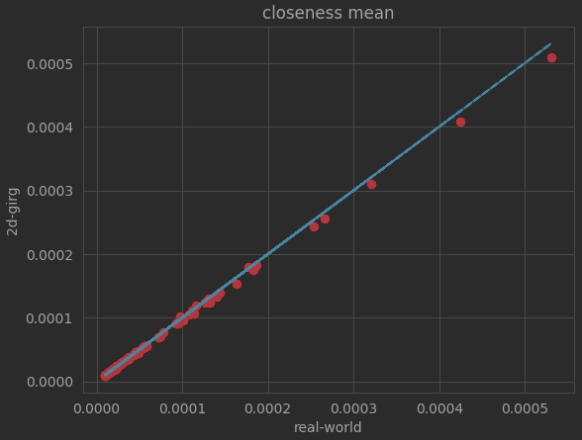
\includegraphics[width=\linewidth]{./figures/real_2d_closeness_mean_scatter.png}
    \caption{2d GIRGs have almost identical mean node closeness to real-world FB graphs}
    \label{fig:real_2d_closeness_mean_scatter}
    \end{subfigure}
    \begin{subfigure}{0.49\textwidth}
    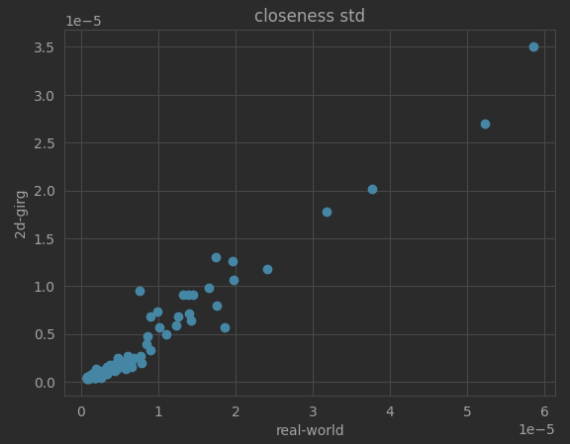
\includegraphics[width= \linewidth]{./figures/real_2d_closeness_std_scatter.png}
    \caption{2d GIRGs have consistently lower standard deviation of node closeness than real-world FB graphs}
    \end{subfigure}
    \begin{subfigure}{0.49\textwidth}
    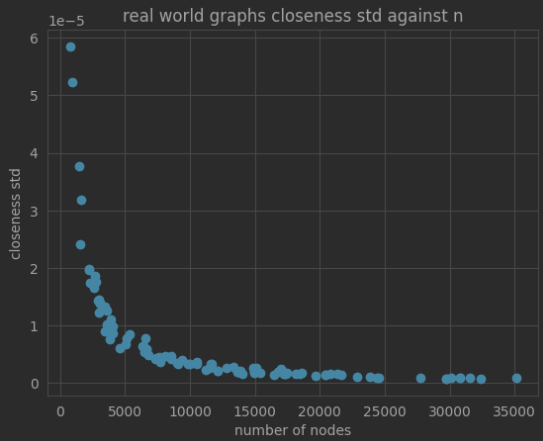
\includegraphics[width=\linewidth]{./figures/real_closeness_std_against_n.png}
    \caption{standrd deviation of node closeness in real-world FB graphs fits well as a function of number of nodes}
    \end{subfigure}
\end{figure}

(cube GIRGs having slightly larger diameters - to get from one edge of the cube to the opposite), but does fit our geometric intuition.


does slightly fit our intuition of their more realistic geometry. Funnily enough Cube GIRGs fit on the dataset have 

just mean that toroidal GIRGs have too large diameters compared to real graph (cube GIRGs having smaller diameters), but does fit our geometric intuition.

2+d min girgs we expect to have very large diameters.




% \begin{sidewaystable}
%     \centering
%     \caption{Feature Set Performance}
%     \begin{tabular}{|l|c|c|c|c|c|c|c|c|c|c|c|c|c|c|c|c|c|c|c|}
%             \hline
%             Features & 1co & 2co & 5co & CL & 1-23 & 1-234 & 1min & 5min & 1cu & 2cu & 3cu & 1 & 2 & 7 & BA & ER & hyper \\ \hline
%             n, m, betw & 81 & 84 & 95 & 95 & 99 & 99 & 99 & 100 & 99 & 100 & 100 & 99 & 99 & 99 & 100 & 100 & 99 \\ \hline
%             n, m, core & 93 & 91 & 91 & 85 & 100 & 100 & 100 & 100 & 100 & 100 & 100 & 100 & 100 & 100 & 100 & 100 & 100 \\ \hline
%             n, m, close & 92 & 86 & 86 & 91 & 99 & 99 & 99 & 97 & 99 & 98 & 95 & 98 & 98 & 98 & 99 & 100 & 97 \\ \hline
%             n, m, c & 95 & 92 & 100 & 100 & 100 & 100 & 100 & 100 & 100 & 100 & 100 & 100 & 100 & 100 & 100 & 100 & 100 \\ \hline
%             n, m, deg & 87 & 77 & 66 & 55 & 100 & 100 & 100 & 100 & 100 & 100 & 100 & 100 & 100 & 100 & 100 & 100 & 100 \\ \hline
%             n, m, Katz & 76 & 75 & 62 & 54 & 94 & 94 & 94 & 91 & 94 & 97 & 99 & 94 & 93 & 94 & 100 & 99 & 94 \\ \hline
%             n, m, PR & 82 & 76 & 77 & 77 & 100 & 100 & 100 & 100 & 100 & 100 & 100 & 100 & 100 & 100 & 100 & 100 & 100 \\ \hline
%             n, m, comm & 97 & 95 & 95 & 91 & 98 & 98 & 98 & 99 & 93 & 95 & 93 & 95 & 96 & 89 & 95 & 90 & 99 \\ \hline
%             n, m, kcore & 94 & 92 & 88 & 84 & 100 & 100 & 100 & 100 & 100 & 100 & 100 & 100 & 100 & 100 & 100 & 100 & 100 \\ \hline
%             n, m, diam & 97 & 98 & 97 & 100 & 100 & 100 & 100 & 100 & 100 & 100 & 100 & 100 & 100 & 100 & 100 & 100 & 100 \\ \hline
%             n, m, e-diam & 78 & 76 & 78 & 89 & 92 & 83 & 83 & 99 & 82 & 77 & 77 & 85 & 83 & 88 & 100 & 99 & 83 \\ \hline 
% \end{tabular}
% \end{sidewaystable}

\begin{sidewaysfigure}
    \centering
    % \begin{subfigure}
    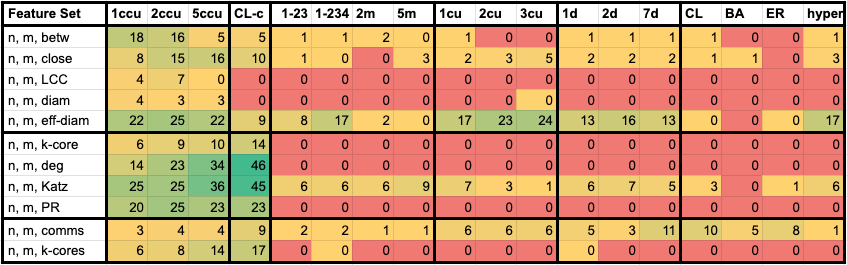
\includegraphics[width=\textwidth]{./figures/Blasius_framework_table.png}
    \caption{\cite{blasius2018towards} GGM comparison framework on Facebook graphs, extended to different GIRG models. Classification accuraciese by SVM use various feature sets. We chose to focus on feature sets involving one core feature (mean, quartile and standard deviation statistics) on top of just number of nodes and edges. If just one of mean/median is used, accuracies are often lower, sometimes even in $50\%-70\%$. $50\%$ is the best possible validation of a GGM as indistinguishable from real data, and is only achieved for feature set $n, m, LCC \;\text{mean}$ (by GIRGs and not the other none geometric GGMs). Some models are missing from the table e.g. 3d-6d GIRGs as their results follow a trend from low to high dimension.
    }
    \label{fig:blasius_framework_table}
    % \end{subfigure}
    \vspace{1em}
    \centering
    % \begin{subfigure}
    \begin{tabular}{|c|c||c|c|}
        \hline
        1-ccu & 1d copy weight cube GIRG 
        & betw & betweenness centrality
        \\
        1-23 & $1 \lor (2 \land 3)$ mixed min/max GIRG
        & k-core & node k-core number
        \\
        2-min & $1 \lor 2$ 2d min GIRG
        & close & closeness centrality
        \\
        3-cu & 3d cube GIRG
        & LCC & node local clustering coefficient
        \\
        7d & 7d GIRG
        & deg & node degree
        \\
        CL & ChungLu
        & Katz & node Katz centrality
        \\
        CL-c & copy weight ChungLu
        & PR & node PageRank
        \\
        BA & Barabasi-Albert
        & comms & community sizes
        \\
        ER & Erdos-Renyi
        & k-cores & k-core sizes
        \\
        hyper & Hyperbolic Random Graph &
        diam & graph diameter
        \\
        && eff-diam & graph effective diameter\\
        \hline
    \end{tabular}
    \caption{Graph Generative Model abbreviations; feature name abbreviations}
% \end{subfigure}
\end{sidewaysfigure}

% \begin{sidewaystable}
%     \centering
%     \begin{tabular}{|c|c|}
%         \hline
%         1-co & 1d copy weight GIRG \\
%         1-23 & $1 \lor (2 \land 3)$ mixed min/max GIRG \\
%         2-min & $1 \lor 2$ 2d min GIRG \\
%     \end{tabular}
% \end{sidewaystable}


% Translating the two equivalent volumetric and distance based formulations of the Toroidal GIRG to the Cube actually gives two different but both potentially sensible definitions. 

% We'll start with the Toroidal Max GIRG where the distance function is $r^\T(x_u, x_v) = \norm{x_u - x_v}_{\infty, \T}$, the derived volume function in the toroidal setting is $Vol^\T(r^\T_{uv}) = (2r^\T_{uv})^d$, and the toroidal edge probability is $p_{uv}(r^\T) = \min \left \{1, \left ( \frac{w_u w_v}{n Vol^\T(r_{uv})} \right )^\alpha \right \} = \min \left \{1, \left ( \frac{w_u w_v}{n (2r^\T_{uv})^d} \right )^\alpha \right \}$. 

% The distance based cube GIRG connection probabilities just replaces $r^\T_{uv}$ with the cube distance $r_{uv}$, which is in general equal, or longer depending on the positions $x_u, x_v$.

% The translation of $Vol^\T(r^\T_{uv})$ into a cube geometry now no longer makes sense without a reference point about which the ball volume is measured. Hence it is replaced with $\sqrt{V_u(r_{uv}) V_v(r_{uv})}$, where $V_u(r_{uv})$ is the volume of the $r_{uv}$ ball about point $x_u$, only including intersection with the cube. This definition partially assuages the reduced connectivity of points $u$ that are near the extremes of the cube - their $V_u(r_{uv})$ is smaller than if they were more centrally located, and hence they strive more strongly to connect - however their potential neighbours $v$ will still usually be more centrally located and hence less willing to reciprocate the connection.

% The upshot connectivity comparison between the Torus and Cube GIRG, is that connection probabilities for centrally located nodes are generally the same. For distance based Cube GIRGs, connection probabilities everywhere are upper bounded by the Toroidal GIRG, and extremely located nodes have fewer neighbours. For volumetric Cube GIRGs, centrally located nodes actually have more neighbours than before, and extremely located nodes have fewer neighbours, but likely not in any balanced fashion.

% connection probability is higher. However it does not fully assuage this, as the volume of the $r_{uv}$ ball about $x_u$ is still smaller than if it were a torus, as the ball is cut off by the cube. 

% using now $p_{uv}(r) = \min \left \{1, \left ( \frac{w_u w_v}{n \sqrt{V_u(r_{uv}) V_v(r_uv)})} \right )^\alpha \right \}$, where now $r_{uv}$ is cube distance - so in general equal or longer than torus distance, and $V_u(r_{uv})$ is the volume of the $r_{uv}$ ball about point $u$, only including intersection with the cube.

% with just the fact that the underlying space is a Cube rather than a Torus changing the connection probabilities. The second is a more direct distance based formulation, $p_{uv}(r) = \min \left \{1, \left ( \frac{w_u w_v}{n r_{uv}^d} \right )^\alpha \right \}$. To be clear, these two formulations are for a given fixed distance function $r_{uv} = r(x_u, x_v) = ||x_u - x_v||_\infty$. 

% The volumetric formulation has the benefit that all nodes have the same expected degree profile no matter their location, whereas for the distance based formulation, a node near the edge of the cube would have fewer neighbours in expectation than if it were more centrally located. The distance based formulation 


\begin{comment}
\section{Weird GIRGs}
The generalisation formula is given by 
\begin{equation}
    p_{uv} = \min \left \{ 
        1,
        c \left (
            \frac{w_u w_v}{Vol(r_{uv})}
        \right )^\alpha    
    \right \}
\end{equation}
Where $r_{uv} = ||x_u - x_v||$. This is in the schema where $Vol(Torus) = n$. This is designed such that a $dV$ section of volume with approximately same radius $r$ from $x_u$ contains about $dV$ points. 


Ooooops
Ok

The whole point is that we want $p(u \sim v | x_u, w_u, w_v) = \Theta(w_u w_v)$ a la Chunglu.
$blah = \int p_{uv}(r) p(r) dr = V(\hat{r}) + \int_{\hat{r}}^{n^{1/d}} p_{uv}(r) p(r) dr$.
Both terms are Theta the same amount. $\hat{r}$ is defined to be the point when $p_{uv}(r) = 1$, i.e. $r = \Theta(w_u w_v)$. You can also see that the second integral fits this too. Since $p(r) = \dot(V)/n$, we get $\int ... p(r) dr = \int (w_u w_v / V)^\alpha dV = (w_u w_v)^\alpha \int 1/V^\alpha dV$. Now $\int_{\hat{V}}^n 1/V^\alpha dV = \hat{V}^{1 - \alpha} = (w_u w_v)^{1- \alpha}$.


This is kind of beautiful. It doesn't really matter what Volume function we use, as long as the volume of the whole Torus is fixed and makes sense (I guess either n or 1). This results in having exactly the same average degree, regardless of MAX GIRG or MIN GIRG or whatever. For the MAX GIRGs, Blasius actually calculated precisely $\E[X_{uv} | w_u w_v]$, via some volume/radius integrals, to get some complex formula s.t. $\E[\bar{d}] = f(c) = c^\alpha (...) + c(...)$, which is then numerically solved to find $\hat{c}: f(\hat{c}) = \text{desiredAvgDegree}$. We can then precisely use this same constant $c$ in our MIN GIRG shenanigans:


MCD GIRGs vs MAX GIRGs average degree.
As far as I can tell, they should have the same avg degree, and this is borne out. Note PointTorus uses $Vol(r) = r^d$ whereas PointTorus2 uses $Vol(r) = (2r)^d$ which is actually the correct volume, and hence a scale factor is used between the two.

Unfortunately this geometric space equivalence only holds on all toroidal geometries, so won't work for CUBE GIRGs I believe.

\begin{verbatim}
    n = 1500
    d = 3
    tau = 2.1
    alpha=1.2
    desiredAvgDegree=100.0
    
    g, edges, weights, pts_torus, const = generation.generate_GIRG_nk(n, d, tau, alpha, desiredAvgDegree=desiredAvgDegree, points_type=points.PointsTorus)
    print(const)
    utils.avg_degree(g)
    print()
    
    g, edges, weights, pts_torus2, _ = generation.generate_GIRG_nk(n, d, tau, alpha, points_type=points.PointsTorus2, weights=weights, const=const*(2**d))
    print(_)
    utils.avg_degree(g)
    print()
    
    g, edges, weights, pts_torus2, _ = generation.generate_GIRG_nk(n, d, tau, alpha, points_type=points.PointsMCD, weights=weights, const=const*(2**d))
    print(_)
    utils.avg_degree(g)

    =============================================

    1.3638471818782616
    100.10933333333334

    10.910777455026093
    100.004

    10.910777455026093
    100.44133333333333

\end{verbatim}

\chapter{GIRG fitting}


\chapter{Classification :(}


% \paragraph{Example Paragraph}
% \subparagraph{Example Subparagraph}
\end{comment}